\documentclass[a4paper]{article}

\usepackage[utf8]{inputenc}
\usepackage{microtype}
\usepackage{enumitem}
\usepackage{comment}
\usepackage{float, graphicx}
\usepackage{mathtools, amssymb}
\usepackage{caption}
\usepackage{subcaption}

\setlength{\parindent}{0em}
\graphicspath{ {../images/} }

\title{5}
\date{}

\begin{document}
\maketitle

\section{Part-a}
Control points were selected as mentioned. Care was taken to select salient features such as easily identifiable points and corners.

\section{Part-b}
The code to calculate the affine matrix can be found inside the code directory. The affine matrix was calculated by using P1 and P2 matrices consisting of control points for image1 and imag2  and finding the pseudo inverse of P1.


\section{Part-c}
The nearest neighbor approximation has been implemented and can be seen in the code section.
The Images are:



\begin{figure}[H]
\begin{subfigure}{.4\textwidth}
  \centering
  % include first image
  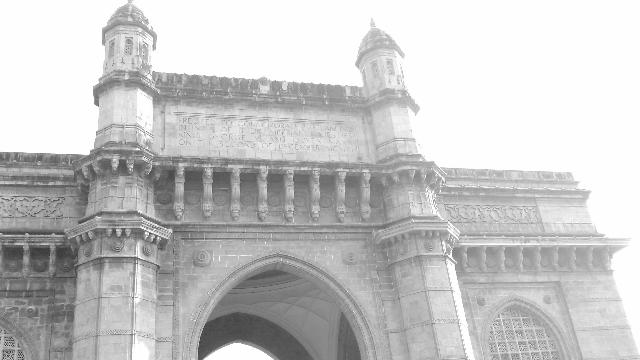
\includegraphics[width=.8\linewidth]{goi1.jpg}  
  \caption{goi1}
  
\end{subfigure}
\begin{subfigure}{.4\textwidth}
  \centering
  % include second image
  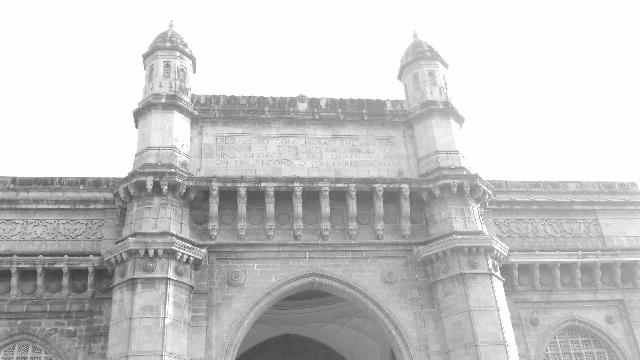
\includegraphics[width=.8\linewidth]{goi2_downsampled.jpg}  
  \caption{goi2}
  
\end{subfigure}



\begin{subfigure}{.4\textwidth}
  \centering
  % include third image
  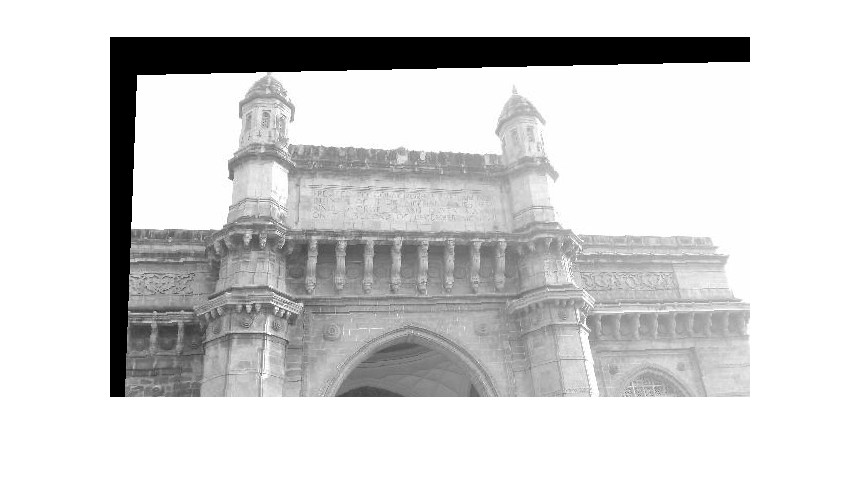
\includegraphics[width=.8\linewidth]{nearest_neighbour.jpg}  
  \caption{nearest-neighbour}
  
\end{subfigure}
\begin{subfigure}{.4\textwidth}
  \centering
  % include fourth image
  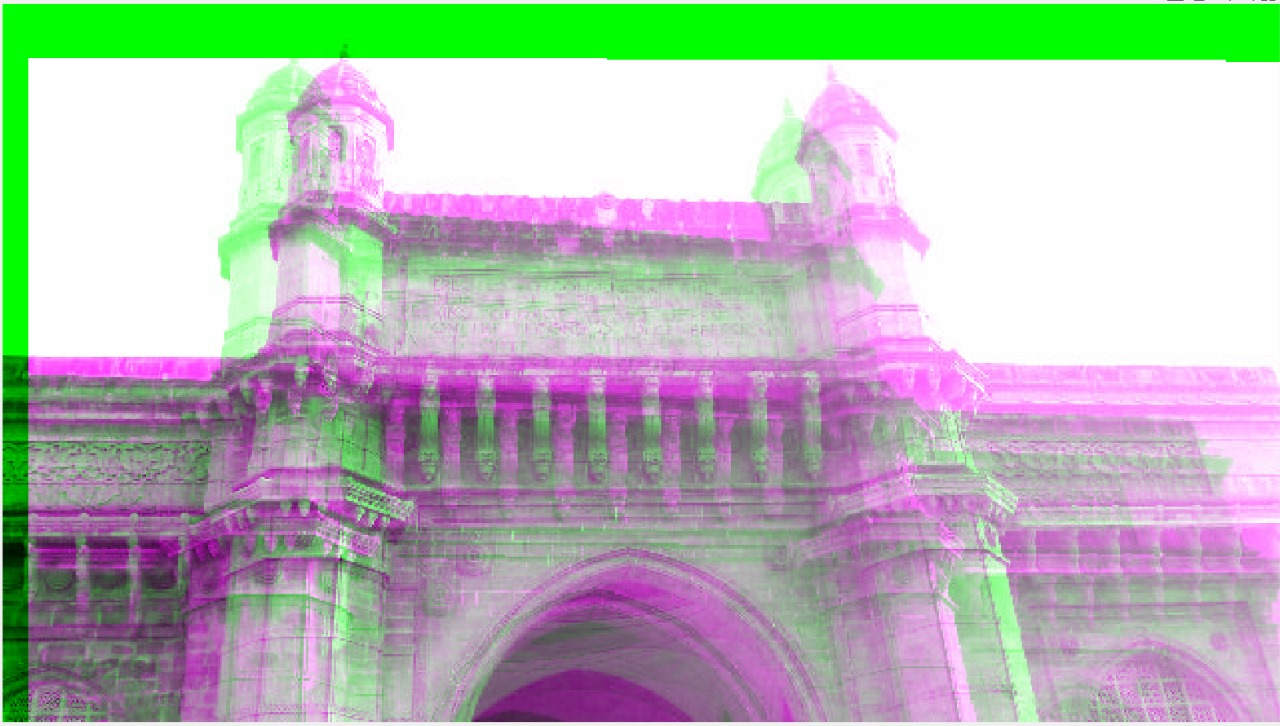
\includegraphics[width=.8\linewidth]{n-12.jpg}  
  \caption{overlay}
  
\end{subfigure}
\caption{Nearest Neighbour}

\end{figure}


\section{Part-d}
The Bi-linear approximation has been implemented and can be seen in the code section.
The Images are:

\begin{figure}[H]
\begin{subfigure}{.4\textwidth}
  \centering
  % include first image
  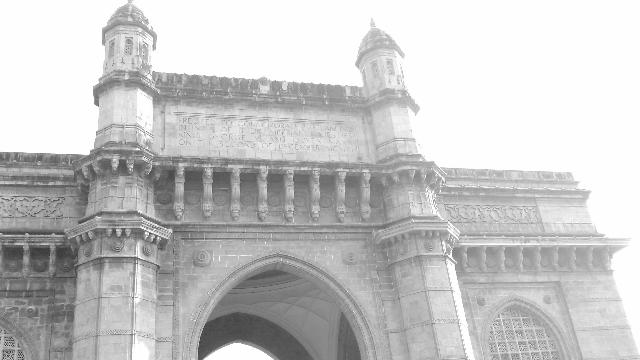
\includegraphics[width=.8\linewidth]{goi1.jpg}  
  \caption{goi1}
  
\end{subfigure}
\begin{subfigure}{.4\textwidth}
  \centering
  % include second image
  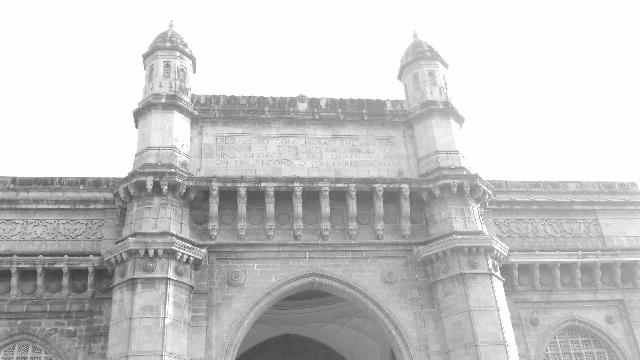
\includegraphics[width=.8\linewidth]{goi2_downsampled.jpg}  
  \caption{goi2}
  
\end{subfigure}



\begin{subfigure}{.4\textwidth}
  \centering
  % include third image
  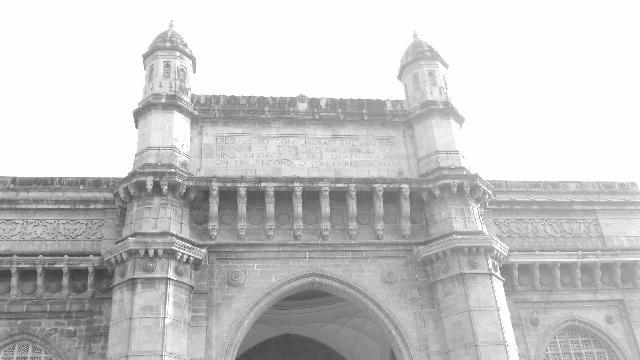
\includegraphics[width=.8\linewidth]{b.jpg}  
  \caption{Bi-linear}
  
\end{subfigure}
\begin{subfigure}{.4\textwidth}
  \centering
  % include fourth image
  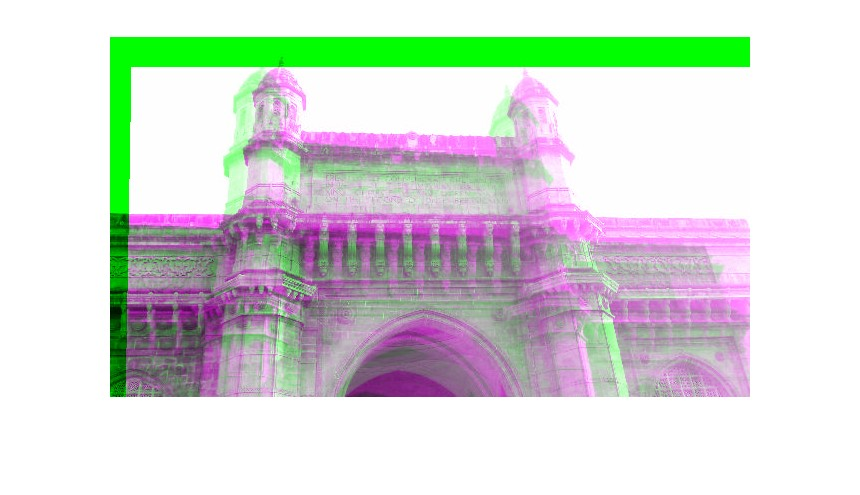
\includegraphics[width=.8\linewidth]{ob.jpg}  
  \caption{overlay}
  
\end{subfigure}
\caption{Bi-linear}

\end{figure}
\section{Part-e} % (fold)
\label{sec:part_e}

Let the matrices of formed by points of image 1 and image 2 be $M_1$ and $M_2$ respectively such as:
\begin{equation}
	M_i =
	\begin{bmatrix}
		x_{i1} & x_{i2} & \cdots & x_{in}\\
		y_{i1} & y_{i2} & \cdots & y_{in}\\
		1 & 1 & \cdots & 1
	\end{bmatrix}
\end{equation}
As the points of first image are collinear, the ratio $x_{1i}:y_{1i}$ is same for all $i$. Also, $x_{1i}$ or $y_{1i}$ can't be zero for any $i$ due to MATLAB's 1-based indexing, so the ratio can't be 0 or undetermined.

Now, $\operatorname{rank}(M_1)\leq 2$. This is because the rank is equal to one only when all $x_{1i}$'s are equal to each other and all $y_{1i}$'s are equal to each other. But this means that all points are same. If any two or $x_{1i}$'s or $y_{1i}$'s are unequal then the first row and last row become linearly independent. Hence, for distinct points $\operatorname{rank}(M_1)=2$ 


We know that the affine model equation with control points is given by:
\begin{equation}
	A\cdot M_1 = M_2% \Rightarrow A = M_1 * M_1^+
\end{equation}
The above equation can be rewritten in terms of a least square system as follows:
\begin{equation}
	\underbrace{
	\begin{bmatrix}
		x_{11} & y_{11} & 1 & 0 & 0 & 0\\
		x_{12} & y_{12} & 1 & 0 & 0 & 0\\
		\vdots & \vdots & \vdots & \vdots & \vdots & \vdots \\
		x_{1n} & y_{1n} & 1 & 0 & 0 & 0\\
		0 & 0 & 0 & x_{11} & y_{11} & 1\\
		0 & 0 & 0 & x_{12} & y_{12} & 1\\
		\vdots & \vdots & \vdots & \vdots & \vdots & \vdots \\
		0 & 0 & 0 & x_{1n} & y_{1n} & 1
	\end{bmatrix}}_{P}
	\begin{bmatrix}
		A_{11}\\A_{12}\\t_x\\A_{21}\\A_{22}\\t_y
	\end{bmatrix}
	=
	\begin{bmatrix}
		x_{21}\\
		x_{22}\\
		\vdots\\
		x_{2n}\\
		y_{21}\\
		y_{22}\\
		\vdots\\
		y_{2n}\\
	\end{bmatrix}
\end{equation}
Clearly the $\operatorname{rank}(P)=2\cdot\operatorname{rank}(M_1)=4$.

We know from linear algebra that the least squares solution is unique iff the columns of a tall matrix $P$ are linearly indepedent. That is the matrix $P$ must be full rank. 

Since, $P$ is not full rank here, this system has infinite solutions for the matrix $A$. 

Hence, if we take collinear points then $A$ is not unique and this might lead to problems while solving for $A$ with different approaches.
% section part_e (end)



\end{document}
